            {\scriptsize \color{AcademicNavy} \textbf{$\Sigma 5$ boundary}} \\[0.2cm]
            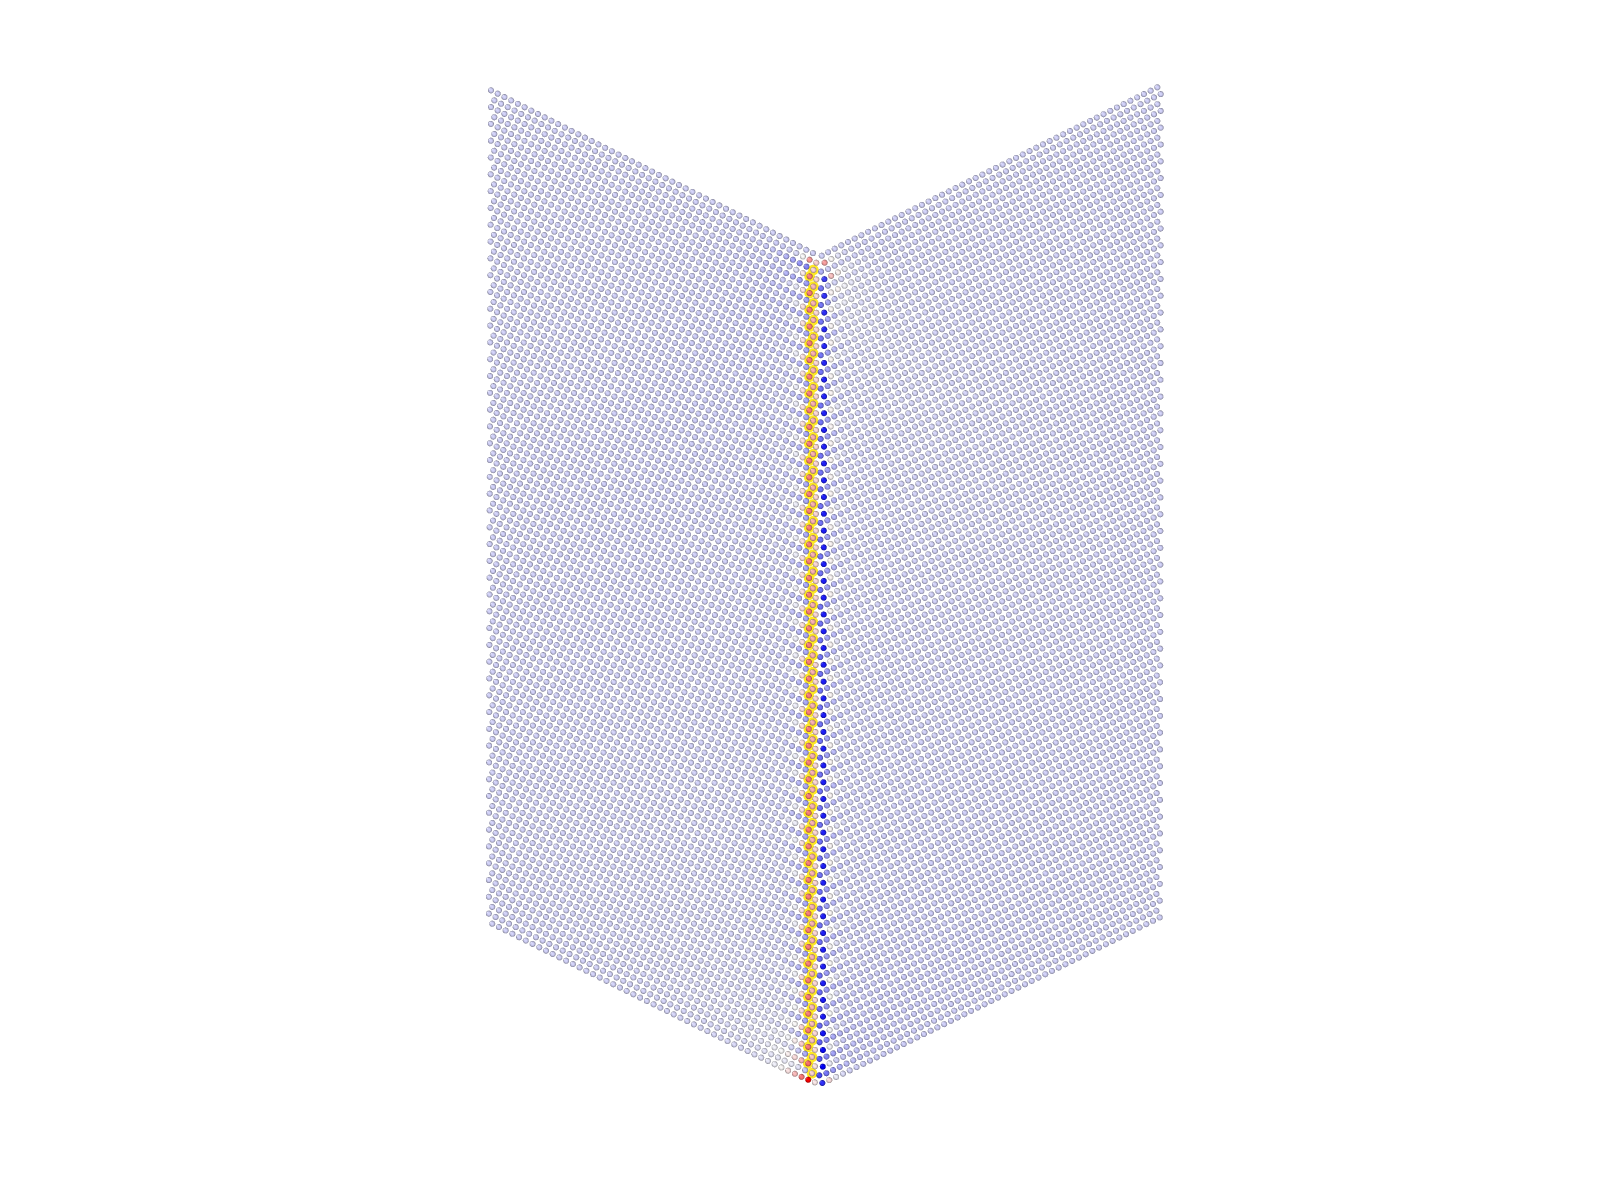
\includegraphics[height=4.8cm, keepaspectratio]{Figures/gb_special_sigma.png}
        \end{column}
    \end{columns}
\end{frame}

% Slide 40: Theoretical Context & Historical Bottlenecks
\begin{frame}{Theoretical Context \& Historical Bottlenecks}
    \begin{itemize}
        \item \textbf{Foundational 1D Models}: Frenkel–Kontorova and Peierls–Nabarro frameworks for defect cores [10, 11].
        \item \textbf{Numerical Transition}: Ginzburg–Landau formalism with periodized energy density for shear/tetragonal strains [12--14].
        \item \textbf{Geometric Hurdles}:
        \begin{itemize}
            \item Cubic finite-difference vs. triangular lattices [12]. 
            \item Inherent bias toward orthogonal slip systems.
        \end{itemize}
        \item \textbf{Structural Bottleneck}: Reliance on \textit{linearized strain measures} prevents capturing lattice rotations and large deformations [15--17].
    \end{itemize}

    \vfill
    {\tiny [10] Kontorova \& Frenkel, JETP (1939) \quad [11] Peierls, Proc. Phys. Soc. (1940) \\
    [12] Onuki, PRE (2003) \quad [13] Onuki et al., Pramana (2005) \quad [14] Minami \& Onuki, Acta Mater. (2007) \\
    [15] Geslin et al., Acta Mater. (2014) \quad [16] Salman \& Truskinovsky, PRL (2011) \quad [17] Salman \& Truskinovsky, IJES (2012)}
\end{frame}

% Slide 41: Nano-indentation
\begin{frame}{Nano-indentation}
    \vspace{0.4cm}
    \begin{columns}[T, onlytextwidth]
        \begin{column}{0.48\textwidth}
            \centering
            {\small \color{AcademicNavy} \textbf{no rebonding}}
        \end{column}
        \begin{column}{0.48\textwidth}
            \centering
            {\small \color{AcademicNavy} \textbf{rebonding}}
        \end{column}
    \end{columns}
    \vspace{0.2cm}
    \begin{center}
        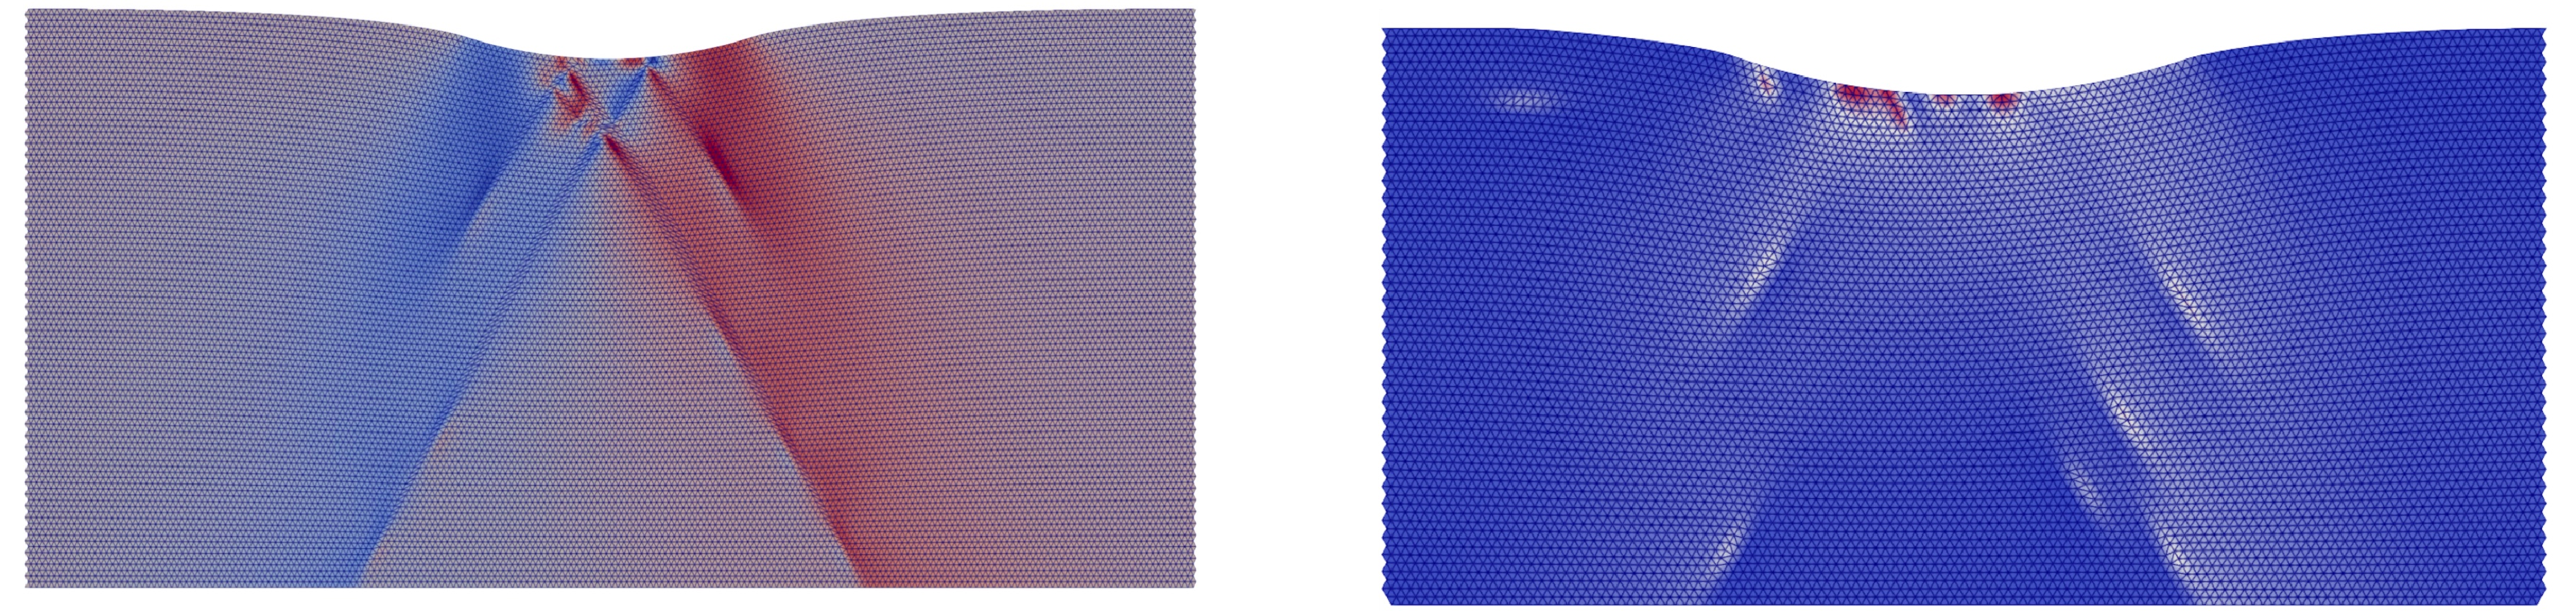
\includegraphics[width=0.95\textwidth, keepaspectratio]{Figures/indentation2.pdf}
    \end{center}
\end{frame}

\end{document}
